\documentclass{article}
\usepackage[utf8]{inputenc}
\usepackage{graphicx}


\title{Computer Architecture Homework 4}
\date{Spring 2019, March}

\begin{document}

\maketitle

\section{Synchronous Finite State Digital Machine Systems}
a. The circuit shown below can be simplified. Write a Boolean expression that represents the function of the simplified circuit using the minimum number of AND, OR, and NOT gate.
\begin{figure}[htbp]
	\centering
	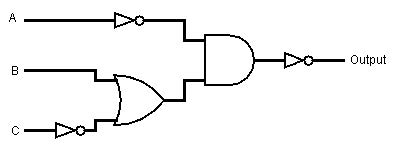
\includegraphics[width=0.7\linewidth]{hw4_1.jpg}
	\label{fig:1}
\end{figure}
\newpage

\noindent b. Consider the finite state machine below which has 6 states and a single input that can take on the value of 0 and 1. The finite state machine should output 1 IF AND ONLY IF 6 + sum of all the input values is not divisible by 2 or 3. One transition has been provided; complete the remainder of the diagram. \\
\noindent (Hint: If the sum of the inputs is a multiple of 6, then we have 6 + sum of the inputs = 6n for some n. As 6n is divisible by 2, 6n cannot be prime.)
\begin{figure}[htbp]
	\centering
	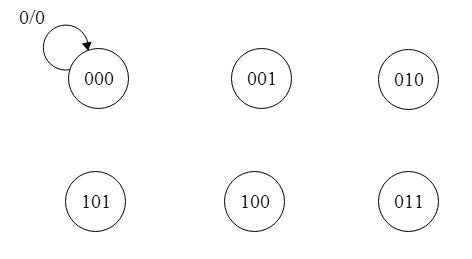
\includegraphics[width=0.7\linewidth]{hw4_2.jpg}
	\label{fig:1}
\end{figure}


\noindent c. Consider the following circuit. Assume registers have a CLK to Q time of 60ps, a setup time of 40ps, and a hold time of 30ps. Assuming that all gates have the same propagation delay, what is the maximum propagation delay each individual gate could have to achieve a clock rate of 1 GHz.
\begin{figure}[htbp]
	\centering
	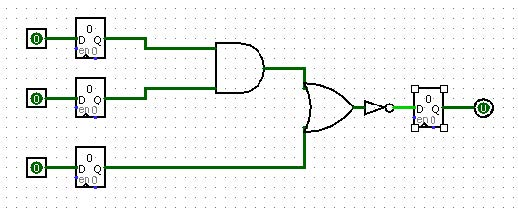
\includegraphics[width=0.7\linewidth]{hw4_3.jpg}
	\label{fig:1}
\end{figure}
~\\
~\\
~\\
~\\
~\\
\newpage
\section{Boolean Logic}
1. Simplify each Boolean expression to one of the following ten expressions:  \\
$0, 1, A, B, AB, A+B, \overline{A} \ \overline{B}, \overline{A}+\overline{B}, A\overline{B}, \overline{A}B$\\
Each answer may be used as many times as necessary.\\
~\\
a.$A(A+\overline{A})+B$
~\\
~\\
~\\
~\\
~\\

\noindent b.$(A+B)(\overline{A}+B)\overline{B}$
~\\
~\\
~\\
~\\
~\\

\noindent c.$\overline{{\overline{A}+\overline{B}}}$
~\\
~\\
~\\
~\\
~\\
\noindent 2. Simplify the following expression step by step (as simple as possible):\\

\noindent a. Standard: $(A+B)(A+\overline{B})C$
~\\
~\\
~\\
~\\
~\\
~\\
~\\

\noindent b. Grouping \& Extra Terms: $\overline{A} \ \overline{B} \ \overline{C}+\overline{A}B\overline{C}+AB\overline{C}+A\overline{B} \ \overline{C}+ABC+A\overline{B}C$
~\\
~\\
~\\
~\\
~\\
~\\
~\\

\noindent c. DeMorgan's: $\overline{A(\overline{B} \ \overline{C}+BC)}$
~\\
~\\
~\\
~\\
~\\
~\\
~\\


\section{Logic Gates}
a. Create a NOT gate using only NAND gates.
~\\
~\\
~\\
~\\
~\\
~\\
~\\
\noindent b. Create an AND gate using only NAND gates.
\noindent (Hint: use a)
~\\
~\\
~\\
~\\
~\\
~\\
~\\
\noindent c. Create an OR gate using only NAND gates.
~\\
~\\
~\\
~\\
~\\
~\\
~\\
\noindent d. Create a NOR gate using only NAND gates.
\noindent (Hint: use a \& c)
~\\
~\\
~\\
~\\
~\\
~\\
~\\

\end{document}
